\subsubsection{Polyglot Programming}
Believe to be first introduced in 2006 by Neal Ford \cite{PolyglotOrigins}.
Polyglot programming is the practice of writing code, for applications, in multiple languages \cite{PolyglotProgTechTarget} as applications are becoming more complex, in design and functionality, different types of problems occur. This is done to add functionality, efficiency and to tackle specific problems \cite{PolyglotMFowler}, to applications, when a single language can't provide everything required. 

For example, building an E-commerce website would likely involve developing the system using: C\#/Java, Python, JavaScript and HTML5. The document formatting language (CSS) and data query language (SQL) could also be used. JavaScript, HTML5 \& CSS would also be used for user Interface design. C\# and/or Java can be used for Object-orientated functionality etc. SQL would be used for database manipulation/interrogation. Python could be used to provide security protection for applications.

The microservice architecture, being a distributed system, can incorporate polyglot programming extensively. Besides the above mentioned, various microservices could be written in different programming languages, to take advantage of functionality only present in them. 

However, including Polyglot Programming into an application is likely to add complexity to the system. Developers will need to learn the range of languages present or teams will need developers proficient in the required languages.
\subsubsection{Polyglot Persistence}
Believed to have been first conceived by Scott Leberknight \cite{PolyglotPersistLeberknight}. Polyglot Persistence is the practice of having various database technologies to store persistent data. With the introduction of NoSQL Databases, and other non-traditional data stores, the move away from using only a Relational Database Management System (RDBMS) to store data began. 

Similar to polyglot programming, the increased complexity of applications also incurs problems when it comes to storing data. As the variety of data to be stored increases, such as big data, the traditional structured RDBMS is not always suitable. Applications may need data to be stored regularly, if there is multiple users using its services at any one time.

NoSQL databases allows for a variety of unstructured data to be store successfully. Data, keeping in context of this project, such as a customer's basket would not be consistent in what it stores - each item in the basket will possibly have different information stored about it. Adding the fact multiple customers will be using an E-commerce web system at the same time, the velocity of data inserts will be potentially be fast and NoSQL Databases (DB's) can handle this well. They provide Horizontal and vertical scaling. Providing greater benefit than most RDBMS which are limited to vertical scaling
As seen in figure \ref{fig:PolyglotPersistence} \cite{PolyglotSerra}:
\begin{figure}[h]
	\caption{Polyglot Persistence Implementation example}
	\label{fig:PolyglotPersistence}
	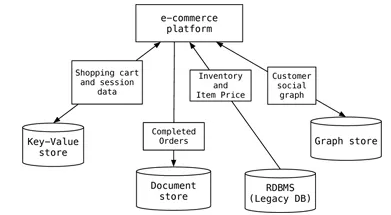
\includegraphics{PolyglotPersistence}
	\centering
\end{figure}

As with Polyglot Programming, Polyglot Persistence adds complexity as each data storage technology added involves learning how they work \cite{PolyglotSerra}.


